\documentclass[12pt]{article}

%Allgemeine Einstellungen

%Abstände
\usepackage[a4paper,left=3cm,right=3cm,top=3cm,bottom=3.5cm,headsep=12pt]{geometry}%Bottom extra 0.5cm für Footer

%Deutsches Sprachpacket
\usepackage[german,ngerman]{babel}

%Times New Roman
\usepackage{mathptmx}

%Titelseite einbinden
\usepackage{pdfpages}

%1.5-Zeilenabstand
\usepackage[onehalfspacing]{setspace}

%Stil der Überschriften, siehe ueberschriften.sty
\usepackage[numeric]{ueberschriften}

%Stil des Inhaltsverzeichnisses, siehe inhaltsverzeichnis.sty
\usepackage[numeric]{inhaltsverzeichnis}

%Abkürzungsverzeichnis, siehe abk_verzeichnis.sty
\usepackage{abk_verzeichnis}

%Stil der Fußzeilen, siehe fusszeilen.sty
\usepackage{fusszeilen}

%Literaturverzeichnis und Zitate, siehe literatur.sty
\usepackage{literatur}

%Stil für Header und Footer, siehe header_footer.sty
%Wenn nicht erwünscht, müssen auch die Befehle \frontmatter, \mainmatter auskommentiert werden
\usepackage{header_footer}

%Stile für Code-Ausschnitte, siehe codes.sty
\usepackage{codes}

%Stile für Anhänge, Bilder, ...
\usepackage{anhang}

%Silbentrennung (manche Worte werden am Zeilenende nicht getrennt, diese müssen dann nachgetragen werden)
\usepackage[T1]{fontenc}
\hyphenation{öf-fent-lich-en}

%DEBUGGING (Zeigt Boxen an)
%\usepackage{showframe}
\setlength{\skip\footins}{12pt}

\usepackage{makecell}
\usepackage{placeins}
\begin{document}

\renewcommand{\mytitle}{Governanceethik und\\moralische Anreize}%Titel für oben links
\renewcommand{\myauthor}{Lennart Schulte-Kellinghaus,\\Timo Stovermann}%Name für unten links
\renewcommand{\headheight}{27pt}%Bei Mehrzeiligem Titel muss Headerhöhe angepasst werden

%
\includepdf[pages={1-}]{titelseite.pdf}
\begin{center}
\LARGE{Governanceethik und moralische Anreize}
\end{center}
\clearpage
\frontmatter%Stil des Headers/Footers ändern

\pagenumbering{Roman}

\renewcommand{\plaintitle}{Tabellenverzeichnis}%Titel für oben Rechts
%Defbox, damit gepunktete Linie bis zur Zahl geht
{\def\makebox[#1][#2]#3{#3}%
	\listoftables 
}

\clearpage

\renewcommand{\plaintitle}{Inhaltsverzeichnis}%Titel für oben Rechts
%Defbox, damit gepunktete Linie bis zur Zahl geht
{\def\makebox[#1][#2]#3{#3}%
	\tableofcontents
}

%\addtocontents{toc}{\vspace{24pt}}%Freiraum im ToC

\clearpage
\mainmatter%Stil des Headers/Footers ändern
\pagenumbering{arabic}

\part{Theoretische Grundlagen}
Ethik spielt in Unternehmen eine immer größer werdende Rolle. Im Kontrast zum 20. Jahrhundert, als beispielsweise hohe Emissionswerte eines Unternehmens kaum Beachtung gefunden haben, gehen die CO\textsuperscript{2}-Emissionen von Unternehmen seit Jahren stetig zurück.\citebib{treibhaus}{}{Vgl. } Genauso hat die Gleichberechtigung von Männern und Frauen immer mehr Präsenz in der Wirtschaft gewonnen, in Form von Anstrengungen den Gender-Pay-Gap zu eliminieren oder den Frauenanteil in Management-Positionen zu erhöhen.\citebib{genderpay}{}{Vgl. } Diese beiden Veränderungen könnten neben vielen anderen maßgeblich durch Ethik bestimmt sein, da sie keinen (direkten) wirtschaftlichen Nutzen schaffen. In wie fern die Ethik und gesellschaftliche wie moralische Aspekte die Entscheidungen eines Unternehmens beeinflussen, soll hier kurz erörtert werden.

\section{Governance}
Gegenüber der klassischen Unternehmensführung versteht man unter dem Begriff Governance nicht-hierarchische Formen der Steuerung, in denen eine Verknüpfung verschiedener Ebenen und Perspektiven im Fokus steht.\citebib{governanceDef}{}{Vgl. } Im wirtschaftlichen Kontext wird der Begriff \textit{Corporate Governance} auf Prinzipien innerhalb eines Unternehmens angewendet, welche den rechtlichen und faktischen Ordnungsrahmen für die Leitung und Überwachung festlegen.\citebib{CODef}{}{} Der Zweck dieser Prinzipien ist es, Interessenkonflikte zwischen Shareholdern und Stakeholdern zu schlichten und das Unternehmen für alle Akteure ansprechend zu gestalten, um opportunistisches Verhalten einzuschränken.\footnote{Vgl. ebd.} Dabei spielen neben ökonomischen auch moralische Anreize eine Rolle.

\section{Die Anreiz-Dimensionen}
Anreize können für Josef Wieland anhand zweier Dimensionen kategorisiert werden, der Art der primären Hintergründe und der Herkunft des Anreizes.\citebib{wielandGMA}{S.14ff.}{Vgl. } Die Hintergründe können ökonomisch sein, also primär auf das Eigeninteresse des Unternehmens bezogen, oder moralisch, welche “nicht nur aufgrund externer Belohnung [...] befolgt”\citebib{wielandGMA}{S.15}{} werden sondern auf gesellschaftlichen Normen basieren. Auf der zweiten Dimension können externe Akteure (Kunden, Partner, Staat, …) oder unternehmensinterne Beweggründe einen Anreiz hervorrufen bzw. belohnen. Daraus ergibt sich eine Matrix mit vier Anreiz-Kategorien.
\begin{table}[h]
\centering
\begin{tabular}{|p{3cm}|p{5cm}|p{5cm}|}
\hline
Anreize & \textbf{extrinsisch} & \textbf{intrinsisch}\\\hline
\textbf{ökonomisch} & extrinsisch-ökonomisch & intrinsisch-ökonomisch\\\hline
\textbf{moralisch} & extrinsisch-moralisch & intrinsisch-moralisch\\\hline
\end{tabular}
\caption{Die Anreizmatrix}
\end{table}

\part{Treiber moralischen Handelns}
Der jeweilige Stellenwert bzw. überhaupt die Existenz der in 1.2 aufgezeigten Kategorien im System der Governance ist unter Ökonomen und Philosophen strittig. Grob lassen sich zwei Sichtweisen erkennen, die monistische und die dualistische.
\section{Die monistische Sichtweise}
Nach der monistischen Ansicht sind die Problemstellungen von Ethik und Ökonomik im Grunde deckungsgleich. Der Soziologe Amitati Etzioni argumentiert, dass moralisches Verhalten nicht auf ein autonomes Anreizsystem zurückführbar sei.\citebib{wielandGMA}{S.5}{Vgl. } Vielmehr sei es gleichermaßen durch ökonomische und moralische Erwartungen bestimmt, die alle auf ökonomische Ziele abgestellt seien. Nach dieser Ansicht wäre der Rückgang von industriellen CO\textsuperscript{2}-Emissionen darauf zurückzuführen, dass die Unternehmen so ihren Kundenkreis sichern und erweitern wollen, da erwartet wird, dass die Kunden die ethische Dimension des Umweltschutzes bei ihrer Kaufentscheidung mit einbeziehen.\\[12pt]
Der Ökonom Karl Homann beschreibt den weitergehenden Standpunkt, dass die Betriebswirtschaftslehre in sich bereits moralisch richtig sei.\citebib{homann}{S.5}{Vgl. } Demnach lägen für fast alle ethischen Probleme ökonomische Rekonstruktionen vor und die Ökonomik sei sogar in der Lage, ethische Probleme zu lösen, da diese in letzter Instanz auch nur auf individuellen Kalkülen basieren. Die Gründe dafür sieht Homann zum einen in der grundlegenden Verschiedenheit von Moral und Wirtschaft, zum anderen in der Beschaffenheit des Menschen als vollständig rational und nutzenorientiert handelnden \textit{homo oeconomicus}.\setlength{\footnotemargin}{4mm}\footnote{Vgl. ebd. S.4}\\
Wenn wir versuchen, die Anreize-Matrix aus 1.3 im monistischen Sinne zu füllen, kommen nur extrinsisch-ökonomische und intrinsisch-moralische Anreize infrage, da sämtliche ökonomisch relevanten Anreize auf eine materielle Vorteilskalkulation zurückführbar sind und der materielle Gewinn durch die externe Partei der Kunden bestimmt wird. Alle immateriellen Anreize beziehen sich demnach auf die Präferenzen der Akteure im Unternehmen und sind ohne monetären Vorteilseffekt sind.
\FloatBarrier
\begin{table}[ht!]
\centering
\begin{tabular}{|p{3cm}|p{5cm}|p{5cm}|}
\hline
Anreize & \textbf{extrinsisch} & \textbf{intrinsisch}\\\hline
\makecell[lt]{\textbf{ökonomisch}} & \makecell[lt]{materiell\\(Gewinnmaximierung,\\ Markenimage, ...)} & \makecell[ct]{-}\\\hline
\makecell[lt]{\textbf{moralisch}} & \makecell[ct]{-} & \makecell[lt]{immateriell\\(Sinn für Gerechtigkeit,\\Überzeugungen, ...)}\\\hline
\end{tabular}
\caption{Die Anreizmatrix aus monistischer Sicht}
\end{table}
\FloatBarrier
\noindent Der Versuch, immaterielle Anreize in die ökonomische Kalkulation mit einzubeziehen, würde demnach nur Rauschen in der Wirtschaft hervorrufen, indem sie für das Wirtschaftssystem irrelevante Diskussionen provozieren.\citebib{wielandGMA}{S.12}{Vgl. }
\section{Die dualistische Sichtweise}
Aus dem Wesen der monistischer Sichtweise folgt, dass sämtliche Handlungen eines (wirtschaftlichen) Akteurs durch andere Akteure bestimmt sind, unabhängig davon, ob sie materieller oder immaterieller Natur sind, da sie alle einen materiellen, monetären Effekt bewirken. Die dualistische Ansatzform geht im Gegensatz dazu davon aus, dass moralische und ökonomische Beweggründe einzeln zu betrachten sind und vor allem nicht immer miteinander einhergehen.\citebib{wielandGMA}{S.6f.}{Vgl. } Als Lösungsansatz für dieses Problem wird in dieser Hausarbeit primär die Governanceethik von Josef Wieland betrachtet, welche ein umfassendes Konzept zur Berücksichtigung genuiner moralischer Anreize in Governancestrukturen liefert.
\subsection{Das Anreizsystem nach Wieland}
Für Wieland beschränken sich moralische Anreize nicht bloß auf die intrinsischen Aspekte, da Achtung und Mißachtung von der Gesellschaft zwar nicht um ihrer selbst Willen verliehen werden aber dennoch moralischer Natur seien.\citebib{wielandGMA}{S.16}{Vgl. } Des weiteren können immaterielle Anreize ebenso von intern heraus entstehen, wie zum Beispiel die Unternehmenskultur.\footnote{Vgl. ebd.}
\FloatBarrier
\begin{table}[ht!]
\begin{tabular}{|p{3cm}|p{5cm}|p{5cm}|}
\hline
Anreize & \textbf{extrinsisch} & \textbf{intrinsisch}\\\hline
\textbf{ökonomisch} & \makecell[lt]{materiell\\(Gewinnmaximierung, ...)} & \makecell[lt]{immateriell\\ (Eigeninteresse, Identität,...)}\\\hline
\textbf{moralisch} & \makecell[lt]{immateriell\\(Achtung, Anerkennung)} & \makecell[lt]{immateriell\\(Sinn für Gerechtigkeit,\\Überzeugungen, ...)}\\\hline
\end{tabular}
\caption{Die Anreizmatrix aus dualistischer Sicht}
\end{table}
\FloatBarrier
\noindent Die vier Anreizformen treten in Wielands System auf unterschiedliche Art in Erscheinung.\citebib{wielandGMA}{S.7}{Vgl. } Extrinsich-ökonomische Anreize sind von außen determinierte, materielle Kalkulationen, wogegen extrinsisch-moralische Anreize nicht auf monetären Zielen sondern auf dem immateriellen Bedürfnis des Menschen nach Anerkennung und Achtung durch Mitmenschen basieren. Die intrinsich-moralischen Anreize stellen die Anreize dar, die befolgt werden um ein inneres Bedürfnis zu erfüllen, und intrinsich-ökonomische Anreize sind interne Anforderungen an das Unternehmen als wirtschaftlichen Akteur, wie zum Beispiel eine Unternehmenskultur oder -identität.
\subsection{Die Bedeutung von Moral in der Wirtschaft}
Die wirtschaftliche wie soziale Gesellschaft besteht aus vielen Teilbereichen, welche teilweise unterschiedliche Ansichten zu den gleichen sozio-ökonomischen Fragestellungen vertreten.\footnote{Vgl. ebd. S.3.} Ein solches Funktionssystem habe jeweils einen Leitcode, eine Sprache über welche es gesteuert wird.\citebib{schneider}{S.1}{Vgl. } Bei der Wirtschaft sei dies der Angebot-Nachfrage-Mechanismus mit dem Kommunikationsmittel Geld, bei der Moral die Wertschätzung, welche unternehmerisches Handeln als gut oder schlecht bewertet. Ein Funktionssystem könne nur über seinen Leitcode kommunizieren, was das Zusammenwirken von mehreren Funktionssystemen zur selben Problematik zunächst unmöglich macht.\citebib{wielandGMA}{S.8}{Vgl. } Daraus folgt, dass die Moral als Zweck an sich im reinen Wirtschaftssystem keinen Platz hat, da sie an sich keine monetäre Wertschöpfung bewirkt. Wieland ist allerdings der Meinung, dass aus institutionsökonomischer Perspektive die moralischen Überzeugungen einer Gesellschaft als integraler Bestandteil der Führung, Steuerung und Kontrolle wirtschaftlicher Transaktionen zu sehen sind.\citebib{schneider}{S.1}{Vgl. } Deshalb wird neben den Funktionssystemen das Konstrukt der Organisationssysteme eingeführt.\citebib{wielandGMA}{S.8}{Vgl. } Diese seien in der Lage, mit mehreren Funktionssystemen zu kommunizieren und Diskurse zwischen diesen zu moderieren. Ein Unternehmen mit moralsensitiven Governancestrukturen ist demnach ein Organisationssystem, welches die Funktionssyteme Wirtschaft und Moral vereint. Jede exakt formulierte und abgrenzbare wirtschaftliche Transaktion hat dann eine moralische und eine ökonomische Dimension, welche vom Organisationssystem \textit{Unternehmen} moderiert werden.
\FloatBarrier
\begin{figure}[ht!]
\centering
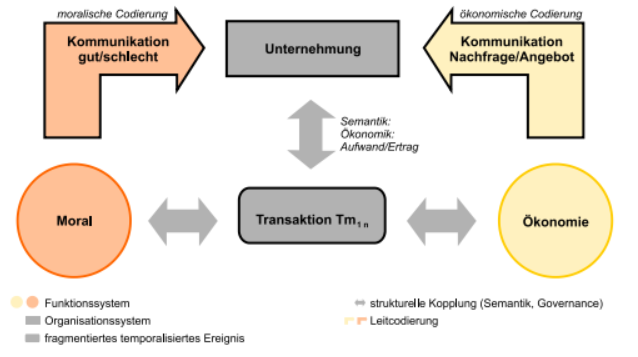
\includegraphics[width=.85\textwidth]{wieland1.png}
\caption{\textit{Schneider, H.}, e-Unternehmensethik (2011), S.1}
\end{figure}
\FloatBarrier
\noindent Neben ökonomischen Gütern, die nach Preis-Leistung kategorisiert und am Markt bewertet werden, gibt es auch moralische Güter, bei denen die moralische Legitimität den Ausschlag gibt.\citebib{wielandGMA}{S.22}{Vgl. } Da sich diese moralischen Güter in ihrer Grundlage von anderen Wirtschaftsgütern unterscheiden und im Zweifelsfall auch ein Stück Kleidung zu einem Moralgut werden kann. Dies wäre zum Beispiel der Fall, wenn bekannt wird, dass die Kleidung mithilfe von Kinderarbeit hergestellt wurde. Deshalb ist es wichtig, dass ein Unternehmen den Umgang mit Moralgütern definiert.\\[10pt]
Die Kernessenz der Moralgüter liegt für Wieland in der sozialen Kooperation von Menschen und Unternehmen.\citebib{wielandGMA}{S.12}{Vgl. } Kein Vertrag und keine Vereinbarung deckt sämtliche Szenarien zu 100\% ab und in eben dieser Unsicherheit kommen extrinsisch-moralische Anreize zum tragen, da diese dem Akteur Achtung und Missachtung für vertraglich nicht geregelte Handlungen zurechnen und so ein Vertrauensverhältnis zwischen Akteuren schaffen.\citebib{gvethWieland}{S.202}{Vgl. } Die intrinsisch-moralischen Güter haben einen Einfluss auf dieses Vertrauensverhältnis, da eigene Überzeugungen, Werte und Haltungen sowie Selbstwertschätzung die Grundlage einer Identitätsbildung seien.\citebib{wielandGMA}{S.20f.}{Vgl. } Diese Identität sei wiederum eine Voraussetzung zur sozialen Kooperation und Kommunikation, über welche Wertschätzung alloziiert werde.\citebib{wielandGMA}{S.20f.}{Vgl. }\\[10pt]
Die Existenzberechtigung der Moral im Wirtschaftssystem nach Wieland ist also die Annahme, dass eine wirtschaftliche Transaktion nicht nur eine materielle Wertsteigerung bewirken soll, sondern auch eine Steigerung der externen und internen Wertschätzung. Um dies umzusetzen, führt Wieland in seiner Governanceethik Wertemanegementsysteme ein.\citebib{wielandGMA}{S.21}{Vgl. } Es sei die Wertesensibilität dieses Governancemechanismus, welche die Befolgung moralischer Anreize ermöglicht. Dabei sei besonders die Implementierung auf Unternehmensebene wichtig, da individuelle Akteure auch durch andere Systeme wie ihre Erziehung oder Religion Wertesensibilität entwickeln.

\subsection{Die Transaktionsformel der Governanceethik}
Um darzustellen, welche Gewichtungen welchen moralischen Gütern in einer wirtschaftlichen Transaktion zukommen, beschreibt Wieland den moralischen Transaktionsmechanismus anhand von vier Einflussfaktoren:\citebib{wielandGMA}{S.11f.}{Vgl. }
\[Tm_{i}=f_{(aIS_i, bFI_{ij}, cIF_{ij}, dOKK_i)}\]
Die Parameter a bis d können jeweils den Wert 1,0 oder -1 annehmen. Der Wert 1 gibt eine positive Wirksamkeit im Hinblick auf die moralische Dimension an. Der Wert -1 gibt genau das Gegenteil an, nämlich eine negative Wirkung auf die moralische Transaktion und der Wert 0 besagt, dass eine Wirkung nicht angenommen wird.\\
Das erste Argument der Formel ist die individuelle Selbstbindung \textit{IS} des Unternehmens, also die o.g. Identität. Ihr Einfluss bestimmt, ob das Ergebnis der Transaktion eher der Tugendethik oder einem rationalem Vorteilskalkül entspricht.\\
Den zweiten Einflussfaktor bilden die formalen Institutionen \textit{FI}. Diese umfassen den gesetzgebenden Staat, Gewerkschaften oder ähnliches.\\
Die informalen Institutionen \textit{IF} bilden das dritte Argument der Formel. Sie umfassen moralische und religiöse Überzeugungen einer gegebenen Kultur. An diesem Argument setzen auch die extrinsisch-moralischen Anreize an, da anhand dieser informalen Institutionen extrinsische Wertschätzung vergeben wird.\\
Den letzten und für die Governanceethik bedeutensten Faktor stellen die Koordinations- und Kooperationsmechanismen des Organsiationssystems \textit{OKK} dar. Darunter sind Leitlinien und Prozesse sowie die Wertemanegementsysteme zu verstehen, mit denen moralische Anforderungen, wie Verzicht auf Kinderarbeit und Korruption operationalisiert und implementiert werden. Sie haben also einen Einfluss auf extrinsisch- und intrinsisch-moralische Anreize, stehen aber gleichzeitig im Konstrukt der Governance im Kontakt zur ökonomisch-intrinsischen und ökonomisch-extrinsischen Perspektive.
\section{Einordnung in philosophische Landschaft}
Die monistische Sichtweise lässt sich gut in den Utiliarismus einordnen, da hier der Gesamtnutzen der Gesellschaft unter der Annahme, dass ökonomisches Verhalten eben dies bewirkt, maximiert werden soll. Mit den Argumenten der Transaktion ergeben sich in der dualistischen Sichtweise folgende Kombinationsmöglichkeiten:\citebib{schneider}{S.10}{Vgl. }
\FloatBarrier
\begin{table}[ht!]
\begin{tabular}{|p{4cm}|p{2cm}|p{2cm}|p{2cm}|p{2cm}|}
\hline
 { } & IS & FI & IF & OKK\\\hline
 Tugendethik & 1 & 0 ; -1 & 0 ; -1 & 0 ; -1\\\hline
 Ordnungsethik & 0 ; -1 & 1 & 0 ; -1 & 0 ; -1\\\hline
 Globale Ethik & 0 ; -1 & 0 ; -1 & 1 & 0 ; -1\\\hline
 Unternehmensethik & 0 ; -1 & 0 ; -1 & 0 ; -1 & 1\\\hline
\end{tabular}
\caption{Ethikformen in der Governanceethik}
\end{table}
\FloatBarrier
\noindent Wenn sich das Handeln an den persönlichen Überzeugungen orientiert, ist das handeln tugendethisch. Ein schlichtes Gehorchen der formalen Institutionen entspricht der Ordnungsethik, welche moralisches Handeln durch Regelsetzung bewirken will. Wenn die globale Gesamtheit moralischer Normen mehr Beachtung als formale Regelungen oder die persönliche Entscheidung bekommt, liegt Globale Ethik vor. Wenn die Governance-Systeme (OKK) die entscheidenend Instanzen darstellen, liegt reine Unternehmensethik vor.\\[10pt]
Die Tugendethik Immanuel Kants besagt im kategorischen Imperativ, dass eine moralische Handlung nicht nur \textit{pflichtgemäß} sein muss, sondern auch \textit{aus der Pflicht heraus} motiviert sein muss. Demnach wäre die Reduktion der CO\textsuperscript{2}-Emmissionen mit dem Ziel der Imagesteigerung keine moralische Handlung, da die Begründung nicht \textit{um ihrer selbst Willen} ist. Wieland sieht hier die Schwäche, dass moralische Handlungen, die aus der reinen Überzeugung, dass sie richtig sind, entstehen, eigentlich auch nur ein Bedürfnis des Menschen stillen sollen, nämlich das, in Einklang mit seinen natürlichen Regungen und dem gesellschaftlichen Habitus zu leben, und somit einen Selbstnutzen mit sich bringen.\citebib{wielandGMA}{S.17}{Vgl. } Zudem sei dieser Habitus nicht naturgegeben, sondern werde über einen sozialen Lernprozess vermittelt. Stattdessen entwickelte Wieland für die Unternehmensethik den organisatorischen Imperativ.\citebib{gvethWieland}{S.197}{Vgl. } Dieser besagt, dass ein Akteur so handeln soll, moralische Güter zu aktivieren und Opportunismus zu minimieren. Das bedeutet, dass moralsensitive Governancestrukturen dafür sorgen müssen, dass die moralischen Anreize genügend Beachtung finden und so opportunistisches Verhalten, wie das Abschließen eines billigen Kaufvertrages über Kleidung aus Kinderarbeit, einzudämmen. In diesem Konstrukt werden Entscheidungen nicht mehr anhand des \textit{homo oeconomicus} getroffen, sondern aus einer situativen Abwägung von Moral und Ökonomie.

\part{Fazit}
Moralisches Handeln ist heutzutage unabdingbar, um am Markt bestehen zu können. Wir sind der Meinung, dass die monistische Sichtweise nicht lang bestehen kann. Nur moralisch zu handeln, um Gewinn zu machen, ist zwar legitim aber irgendwann nicht mehr durchsetzbar, da zum einen Stakeholder und Kunden solch ein Handeln durchschauen und anprangern könnten. Beispielsweise kaufen viele Kunden Lebensmittel nicht aufgrund des Preises sondern, weil sie aus BIO-Produktionen stammen, und gegebenenfalls kehren Mitarbeiter ihrem Arbeitgeber den Rücken, wenn dessen Handeln nicht mit ihrem persönlichen Wertevorstellungen einhergeht. Zum andern sehen wir es wie Wieland aber auch als wichtig an, moralische Werte auf ehrliche Weise im Unternehmen zu verankern. Nur so können ehrliche Zusammenarbeit und ehrliche Kundenbeziehungen entstehen. Wenn ein Unternehmen seine Entscheidungen immer an gerade aktuellen Trends orientiert, ist keine ehrliche Kommunikation möglich, da man als Partner oder Kunde nicht einschätzen kann, ob die Aussagen des Akteurs ehrlich oder nur Fassade sind. Deshalb ist unser Meinung nach die dualistische Sichtweise auch auf lange Sicht gesehen die richtige Art moralisches Handeln in die Wirtschaft einzubetten. Die relevanten Einflussfaktoren überschreiten natürlich die in dieser Hausarbeit angesprochenen Punkte, jedoch bietet Wielands Governanceethik aus unserer Sicht vielversprechende Ansätze, Dialoge zwischen diesen Einflussfaktoren möglichst effektiv zu gestalten.


\clearpage
\frontmatter%Stil des Headers/Footers ändern
\renewcommand{\plaintitle}{Literaturverzeichnis}
\pagenumbering{Roman}
\setcounter{page}{3}
\addtocontents{toc}{\vspace{24pt}}
\addcontentsline{toc}{part}{Literaturverzeichnis}%Literatur-Verz. ins Inhaltsverzeichnis
\printMyBibliography

\end{document}